\documentclass{article}
\usepackage[utf8]{inputenc}
\usepackage{graphicx}

\title{\texttt{manipulator} library for \textbf{Maxima} CAS}

\author{Stanislav Mikhel}
\date{2021}

\begin{document}

\maketitle

\section{About} 

The \texttt{manipulator} library is developed for working with kinematic trees such as robotic manipulators in the \textbf{Maxima} computer algebra system. It is focused on generation of ``raw'' equations, additional simplification of result can be done later if needs. The library allows to do the following operations: 
\begin{itemize}
    \item define the kinematic tree structure manually or import it from URDF file 
    \item solve forward kinematics problem, find the Jacobian 
    \item solve inverse dynamics problem, find matrices M, C and G 
    \item visualize robot structure and print the tree structure 
    \item use different parameterization for rotations
    \item save result in form of \textbf{Matlab} or \textbf{C} code
\end{itemize}

\section{Creating a robot model} 

\subsection{Kinematic tree} 

The library deals with tree-like structures, which represent a sequence of links connected via joints. Each joint can be connected to only one link, but a link can have several joints (Fig. \ref{fig:kinematic_tree}). A joint can be fixed, rotational (revolute) or translational (prismatic). A link can be real (with inertial parameters) or virtual.  The proper tree model in this library must begins with the joint element. 
% can I change it? 

\begin{figure}[t]
    \centering
    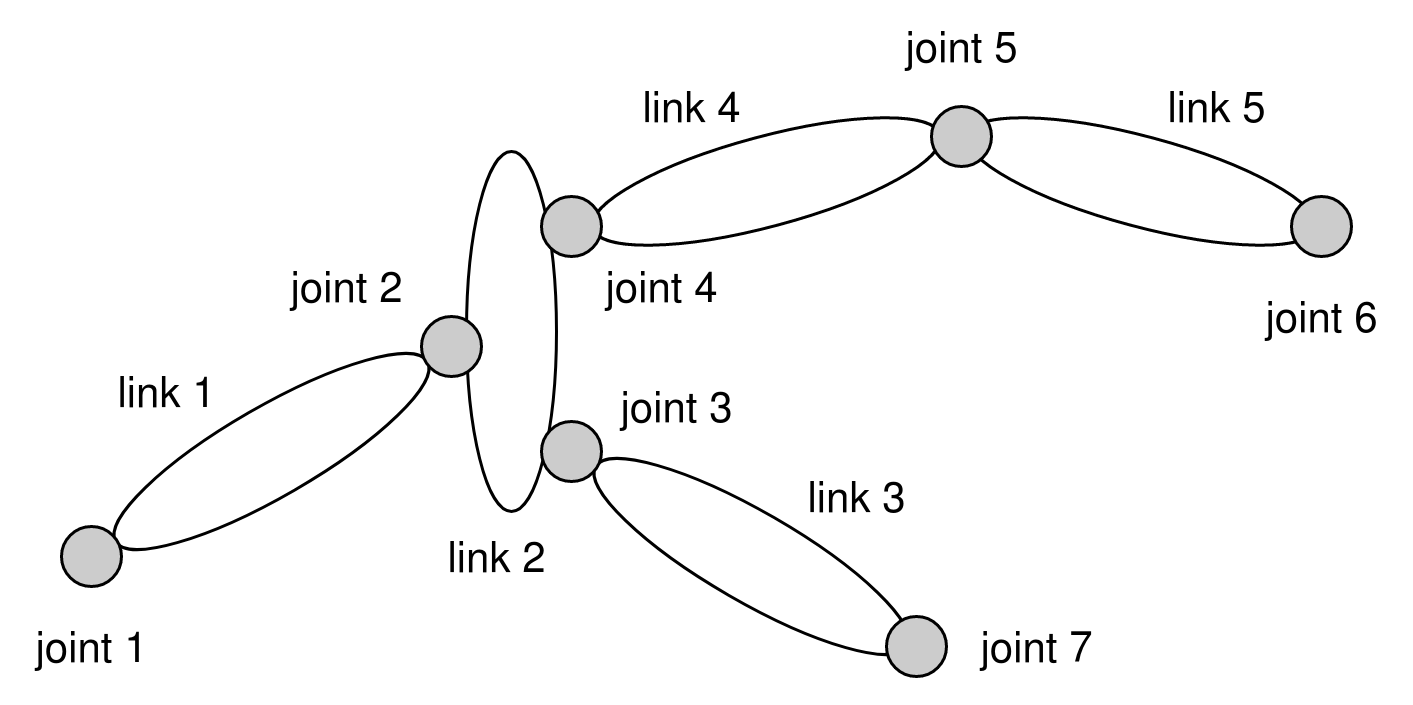
\includegraphics[width=0.8\linewidth]{img/tree_struct.png}
    \caption{Kinematic tree example.}
    \label{fig:kinematic_tree}
\end{figure}

\subsection{Explicit tree structure definition} 

The user can explicitly define links and joints and connect them to make tree. This method is the most flexible but time-consuming technique.  

Links and joints are defined in form of the \textbf{Maxima} structures. Each joint object stores information about its location with respect to the previous joint and indexes of predecessor, successor and the object itself (\texttt{id}). If the join is movable, it includes function of transformation and torque value.  

The joint can be defined with function \texttt{Joint}. It takes 3 arguments: the first one is a transformation function, the second and third are rotation and position or the joint in the previous joint frame, the rotation is a matrix and position is a vector. 
The function of transformation defines not only the type of motion (such as \texttt{rotx} or \texttt{tranz}) but also the name of the joint angle and its derivatives. For example, it you define transformation function as \texttt{rotz(q1)}, then the joint velocity and acceleration called \texttt{dq1} and \texttt{ddq1} respectively. If you want to skip any argument of the transformation function, just use empty list, for example, \texttt{Joint([],[],[])} creates fixed joint with a unit transformation matrix and zero translation vector. 

The link structure stores information about the object \texttt{id}, its predecessor and list of successors. If can additionally contain list of 10 inertial parameters:
\begin{itemize}
    \item $I_{xx}, I_{xy}, I_{xz}, I_{yy}, I_{yz}, I_{zz}$ - elements of the inertia tensor 
    \item $r_{mx}, r_{my}, r_{mz}$ - position of mass center w.r.t. to parent joint
    \item $m$ - mass of the link
\end{itemize}
The link can be created using function \texttt{Link}, that takes the list of inertial parameters of the empty list in the case of virtual link. 

Links and joints can be connected with the help of function \texttt{add\_child}. It is more convenient to use the infix operator ``\texttt{++}''. It returns pointer to the last term that allows to connect a long chain of sequential elements. When you connect link to link or joint to joint, the intermediate element (virtual joint or link respectively) is generated automatically.  

Pointer to the object (link or joint) can be obtained using function \texttt{by\_id} if the object \texttt{id} is known. If the joint variable is known, the corresponding joint can be found with the help of \texttt{by\_name} function. 

\subsubsection{Example: making tree}

The following code allows to create the sequence shown in figure \ref{fig:kinematic_tree} and print its structure. All the link here can be defined implicitly except the ``link2'' that is required to make the second branch. 
\begin{verbatim}
lnk2 : Link([])$ 
/* Save pointer to the last joint */
seq : Joint([],[],[]) ++ Joint([],[],[]) ++ lnk2 
   ++ Joint([],[],[]) ++ Joint([],[],[]) ++ Joint([],[],[])$
/* Add second branch */
lnk2 ++ Joint([],[],[]) ++ Joint([],[],[])$
/* Show the structure */
print_tree(seq);
\end{verbatim}

\subsubsection{Example: 3 link manipulator}
\label{ex:3link}

Let us define structure of a simple 3-link manipulator. Figure \ref{fig:3_links} shows its initial initial configuration. Inertial parameters here are calculated using auxiliary functions from the file \textit{inertia.mac}.  

\begin{figure}[t]
    \centering
    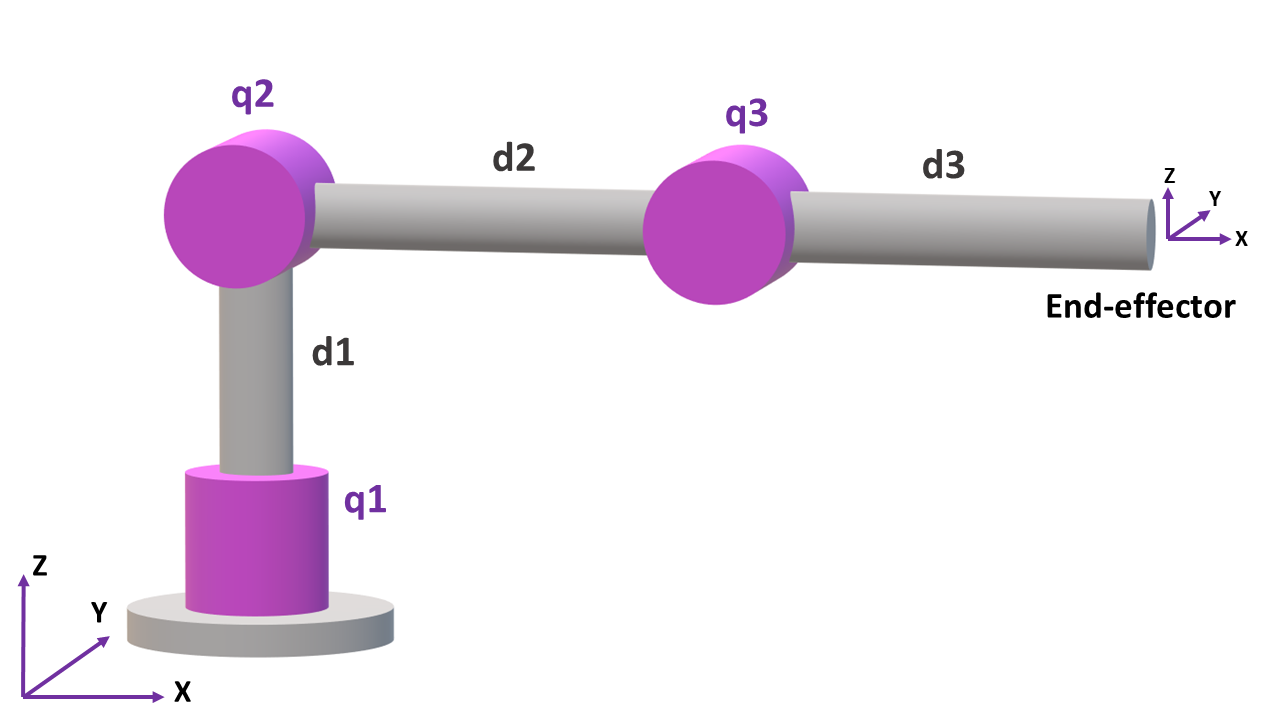
\includegraphics[width=0.8\linewidth]{img/scheme_jnt.png}
    \caption{Manipulator with 3 links.}
    \label{fig:3_links}
\end{figure}

\begin{verbatim}
/* link parameters: length, external and internal radius, m */
d1 : 0.3; r1e : 0.03; r1i : 0.02;  /* 1st */
d2 : 0.5; r2e : 0.03; r2i : 0.02;  /* 2nd */
d3 : 0.5; r3e : 0.02; r3i : 0.015; /* 3rd */
rho : 2700;  /* kg/m^3, alluminium */
/* links */
lnk1 : Link(inertia_cylinder_z(d1,r1e,r1i,rho))$
lnk2 : Link(inertia_cylinder_x(d2,r2e,r2i,rho))$
lnk3 : Link(inertia_cylinder_x(d3,r3e,r3i,rho))$
/* joints */
jnt1 : Joint(rotz(q1),[],[])$
jnt2 : Joint(roty(q2),[],Pos(0,0,d1))$
jnt3 : Joint(roty(q3),[],Pos(d2,0,0))$
ee  : Joint([],[],Pose(d3,0,0))$
/* connect */
rbt : jnt1 ++ lnk1 ++ jnt2 ++ lnk2 ++ jnt3 ++ lnk3 ++ ee$
/* find elements */
by_id( lnk1@id );   /* the same as "lnk1" */
by_name(q2);        /* the same as "jnt2" */
\end{verbatim}

\subsection{List of transformations}

You can use the known sequence of transformations along the manipulator to define its structure with the help of \texttt{from\_list} function. It has two arguments, the first one is the list of transformations, while the second is the list of joint names. The first argument can include any number of translations and rotations with variable or constant parameters. Sequential constant matrices are multiplied to simplified the result. The list of arguments allows to additional parameters in the robot structure. 

\subsubsection{Example: list of transformations} 

Kinematical structure of the manipulator (Ex. \ref{ex:3link}) can be defined as follows. 

\begin{verbatim}
seq : [rotz(q1),tranz(0.3),roty(q2),tranx(0.5),
       roty(q3),tranx(L)]$  /* last length is a parameter */
rbt : from_list(seq, [q1,q2,q3])$
\end{verbatim}

\subsection{Denavit-Hartenberg convention}

If you prefer DH convention for the manipulator description, send it to the function \texttt{from\_dh}. The order of parameters for each link is following: translation in X ($a$), rotation around X ($\alpha$), translation in Z ($d$), rotation around Z ($\theta$). 

\subsubsection{Example: list of DH parameters}

Let us rewrite kinematic structure of Ex. \ref{ex:3link} using DH parameters.

\begin{verbatim}
seq : [
/*  a  alpha    d theta */
 [  0,-%pi/3, 0.5,   q1],   
 [0.5,     0,   0,   q2],  
 [  L,     0,   0,   q3]    /* length is a parameter */
];
rbt : from_dh(seq, [q1,q2,q3])$
\end{verbatim}

\subsection{URDF file}

Universal Robot Description Format (URDF) is a popular XML-based file format for robot description. The \texttt{manipulator} includes \textit{fromxml.mac} library with simple XML parser that allow to deal with valid URDF files. If you don't want to deal with ``raw'' XML node, use function \texttt{from\_urdf}. 

\subsubsection{Example: read URDF}

Assume, you want to read file from the \textit{tests} directory. Then just call the function.
\begin{verbatim}
rbt : from_urdf("tests/3links.urdf")$
\end{verbatim}

\section{Main operations}

Definition of the kinematic tree structure does not includes any additional operations other that element connection. For further analysis you have to use additional functions. Almost in any case the first procedure should be \texttt{update\_state}. It calculates the kinematic relations between the tree components. Argument of this function is any joint of the robot (if you defined the manipulator using any \texttt{from\_} function, it is the last joint). 

\subsection{Forward kinematics}

For each joint you can call function \texttt{get\_pos} to get the position vector of this joint in the robot base frame. Likewise, the \texttt{get\_rot} returns the joint rotation matrix. 

\subsubsection{Example: FK}

For the manipulator (Ex. \ref{ex:3link}) we can solve FK problem. 

\begin{verbatim}
/* calculate kinematics */
update_state(rbt); 
/* get joint position as expression */
get_pos(jnt2); 
/* find rotation for some joint state */
ev(get_rot(jnt2), q1:%pi/4, q2:%pi/3);
\end{verbatim}

\subsection{Differential kinematics}

The Jacobian allows to connect velocity of end-effector (or other part of the robot) with the rate of change in joint space. Use function \texttt{Jacobian} to calculate it.  

\subsubsection{Example: Jacobian} 

Continue to work with Ex. \ref{ex:3link}.
\begin{verbatim}
/* find Jacobian for the robot end-effector */
jac : Jacobian(rbt)$
/* numerical evaluation */
res : ev(jac, q1:%pi/2, q2:%pi/3, q3:%pi/4);
\end{verbatim}

\subsection{Inverse dynamics}
\label{sec:dyn}

Dynamics calculation in the \texttt{manipulator} is based on the recursive Newton-Euler algorithm and implemented in the function \texttt{update\_dynamics}. It uses the results of \texttt{update\_state} evaluation and have to be called only when the kinematic tree was created. To extract the joint torque expression for some joint from the tree structure one can call function \texttt{get\_torque}.

\subsubsection{Example: dynamics} 

Assume, that in the \ref{ex:3link} we didn't call the method \texttt{update\_state}. 
\begin{verbatim}
/* find kinematics */
update_state(rbt)$
/* find dynamics */
update_dynamics(rbt)$
/* define parameters */
par : [q1=0.1,dq1=0.5,ddq1=1,q2=-0.2,dq2=0.5,ddq2=1,
       q3=0.3,dq3=0.5,ddq3=1,grav=9.81]$
/* find torques */
res : ev([get_torque(jnt1),get_torque(jnt2),
          get_torque(jnt3)],par)$
\end{verbatim}

\subsection{Dynamics matrices} 

The results, obtained in the section \ref{sec:dyn} can be transformed into the matrix representation with the help of function \texttt{M\_C\_G\_J}. It returns list with four elements: the inertia matrix, the matrix of Coriolis and centrifugal terms, vector of gravity components and the list of joints that corresponds to the sequence of elements in the found matrices. 

\subsubsection{Example: matrices} 

Assume that \texttt{update\_dynamics} has been called previously.
\begin{verbatim}
/* find matrices */
[M,C,G,jnts] : M_C_G_J(rbt)$
/* check the result */
/* get velocities */
dqs : makelist(get_dq(x),x,jnts)$
/* get accelerations */
ddqs : makelist(get_ddq(x),x,jnts)$
/* must be equal to the previous result */
res : ev(M . transpose(ddqs) + C . transpose(dqs) + G, par)$
\end{verbatim}

\subsection{Drawing}

Use the function \texttt{draw\_tree} to plot the robot structure. It takes two arguments: the robot object and the list of joint angles. If the joint list is empty (or some angles are skipped) they assumed to be zero. 

\subsubsection{Example: drawing}

Let us visualize the manipulator in the Ex. \ref{ex:3link} when the first joint is $\pi/6$, the second is $\pi/4$, and the third is $-\pi/4$. Assume that \texttt{update\_state} method has been called. The result is shown in Figure \ref{fig:drawing}. Red, green and blue lines correspond to X, Y and Z respectively.
\begin{verbatim}
draw_tree(rbt,[q1=%pi/6,q2=%pi/4,q3=-%pi/4]);
\end{verbatim}

\begin{figure}[t]
    \centering
    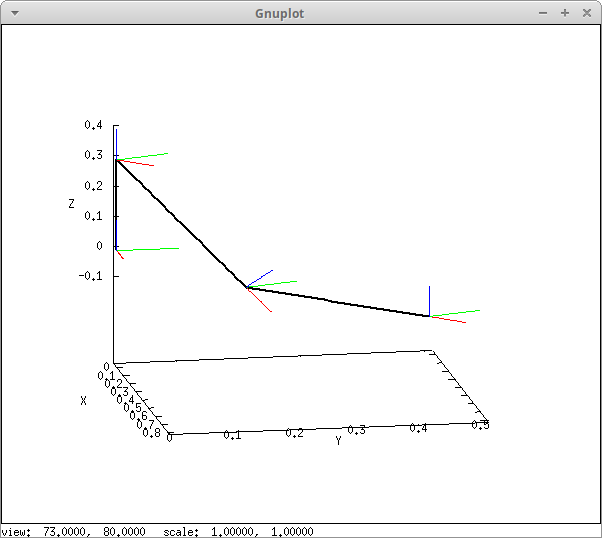
\includegraphics[width=0.8\linewidth]{img/robot_state.png}
    \caption{Robot drawing.}
    \label{fig:drawing}
\end{figure}

\section{Rotations}

The \texttt{manipulator} package contains methods for transformation between different object orientation descriptions. These functions are located in the \textit{rotations.mac} file. The main form of the orientation description in this package is $3 \times 3$ rotation matrix. It can be used in both numerical and symbolical forms. Other parameterisation methods, such as Euler angles, quaternions or pairs of axis and angle can be found from the matrix representation numerically only.  

\subsubsection{Example: rotations} 

\begin{verbatim}
/* get some matrix */
R : Rx(random(1.0)) . Ry(random(1.0)) . Rz(random(1.0));
/* Euler angles in form Y-Z-Y, 2 solutions */
[v1,v2] : R2Euler(R_YZY, R);
/* axis - angle, also 2 solutions */
[v1,v2] : R2AA(R);
/* quaternion */
qu : R2Qu(R);
\end{verbatim}

\section{Export}

The obtained result (matrix, list or variable) can be saved in file if form of \textbf{Matlab} function or \textbf{C} expression using functions from the \textit{save\_as.mac} file. After the function call in your directory will appear the file with name \texttt{get\_}\textit{varname} and the extension \textit{c} or \textit{m}. 

\subsubsection{Example: saving}

Assume that you got matrix $foo$ that you would like to save.
\begin{verbatim}
/* save as a Matlab function 'get_Foo'*/
save_as_matlab("Foo", foo);
/* save as a C array with name 'Foo' */
save_as_c("Foo", foo);
\end{verbatim}

\section{Inertial parameters}

There are some auxiliary functions for calculation the inertia parameters of simple bodies, defined in the \textit{inertia.mac} file. They allows to find elements of the inertia tensor, total mass and center of gravity location based on geometric parameters and the material density. Only two types of the robot links are assumed here: cylinders and cuboids, and the parameters are calculated with respect to the edge with lower coordinate. 

\subsubsection{Example: inertial parameters}

\begin{verbatim}
/* cylindrical link along Y axis, length 0.5m */
/* aluminium, radius exter 0.05m, inter 0.03m */
L : inertia_cylinder_y(0.5, 0.05, 0.05, 2700);
/* full beam in X, length 0.3m, size 0.03m, aluminium */
L : inertia_beam_x(0.3, 0.03, 0, 2700);
\end{verbatim}

\section{List of functions} 

\subsection{manipulator.mac}

\begin{itemize}
    \item \texttt{add\_child(v1,v2)} - make tree by connecting the two given elements (equal to ``v1 ++ v2'')
    \item \texttt{by\_id(n)} - find object by its identifier $n$
    \item \texttt{by\_name(obj,q)} - find joint using the position variable name
    \item \texttt{Cross(v1,v2)} - cross-product of two vectors
    \item \texttt{draw\_tree(obj,qs)} - plot the robot structure for the given joint angles 
    \item \texttt{find\_base(obj)} - find the first element of the tree
    \item \texttt{from\_dh(lst,vars)} - define the serial structure using list of DH parameters in form [$a$, $\alpha$, $d$, $\theta$]
    \item \texttt{from\_list(lst,vars)} - define the serial structure using list of transformation functions and list of variables
    \item \texttt{from\_urdf(name)} - make the robot using URDF file
    \item \texttt{get\_axis(jnt)} - get axis of the joint transformation
    \item \texttt{get\_joints(obj)} - get the list of movable joints in the tree
    \item \texttt{get\_pos(jnt)} - get position vector
    \item \texttt{get\_q(jnt)} - get position variable name 
    \item \texttt{get\_dq(jnt)} - get velocity variable name 
    \item \texttt{get\_ddq(jnt)} - get acceleration variable name
    \item \texttt{get\_rot(jnt)} - get rotation matrix
    \item \texttt{get\_torque(jnt)} - get joint torque value 
    \item \texttt{Homo(fn)} - get equal homogeneous transformation matrix for the given function
    \item \texttt{Jacobian(jnt)} - find the Jacobian matrix from base to the given joint
    \item \texttt{Joint(fn,rot,pos)} - make joint structure using function of transformation $fn$, rotation matrix $rot$ and deflection $pos$ with respect to the previous joint
    \item \texttt{jointp(obj)} - check if the object is joint
    \item \texttt{Link(par)} - make link structure using the given inertial parameters $par$ = [$I_{xx}$, $I_{xy}$, $I_{xz}$, $I_{yy}$, $I_{yz}$, $I_{zz}$, $r_x$, $r_y$, $r_z$, $m$]
    \item \texttt{linkp(obj)} - check if the object is link
    \item \texttt{M\_C\_G\_J(obj)} - get dynamic matrices 
    \item \texttt{movablep(jnt)} - check if the object is movable
    \item \texttt{Pos(x,y,z)} - get vector of arguments
    \item \texttt{print\_tree(obj)} - print the tree structure
    \item \texttt{prismaticp(jnt)} - check if the joint is prismatic 
    \item \texttt{revolutep(jnt)} - check if the joint is revolute
    \item \texttt{rotx(q)} - transformation function for rotation in X
    \item \texttt{roty(q)} - transformation function for rotation in Y
    \item \texttt{rotz(q)} - transformation function for rotation in Z
    \item \texttt{tranx(q)} - transformation function for translation in X
    \item \texttt{trany(q)} - transformation function for translation in Y
    \item \texttt{tranz(q)} - transformation function for translation in Z
    \item \texttt{update\_dynamics(obj)} - find the dynamic equations for all joints
    \item \texttt{update\_state(obj)} - find kinematic equations for all joints 
\end{itemize}

\subsection{rotations.mac}

\begin{itemize}
    \item \texttt{R\_AA(k,q)} - get rotation matrix from the axis $k = [x,y,z]$ and angle $q$ 
    \item \texttt{R\_Qu(v)} - get rotation matrix from the quaternion elements $v = [w,x,y,z]$
    \item \texttt{R\_RPW(r,p,w)} - get rotation matrix from the roll-pitch-yaw angles 
    \item \texttt{R\_XYZ(a,b,c)} - get rotation matrix from Euler angles a,b,c for X-Y-Z axes 
    \item \texttt{R\_XYX(a,b,c)} - get rotation matrix from Euler angles a,b,c for X-Y-X axes
    \item \texttt{R\_XZX(a,b,c)} - get rotation matrix from Euler angles a,b,c for X-Z-X axes
    \item \texttt{R\_XZY(a,b,c)} - get rotation matrix from Euler angles a,b,c for X-Z-Y axes
    \item \texttt{R\_YXY(a,b,c)} - get rotation matrix from Euler angles a,b,c for Y-X-Y axes
    \item \texttt{R\_YXZ(a,b,c)} - get rotation matrix from Euler angles a,b,c for Y-X-Z axes
    \item \texttt{R\_YZX(a,b,c)} - get rotation matrix from Euler angles a,b,c for Y-Z-X axes
    \item \texttt{R\_YZY(a,b,c)} - get rotation matrix from Euler angles a,b,c for Y-Z-Y axes
    \item \texttt{R\_ZXY(a,b,c)} - get rotation matrix from Euler angles a,b,c for Z-X-Y axes
    \item \texttt{R\_ZXZ(a,b,c)} - get rotation matrix from Euler angles a,b,c for Z-X-Z axes
    \item \texttt{R\_ZYX(a,b,c)} - get rotation matrix from Euler angles a,b,c for Z-Y-X axes
    \item \texttt{R\_ZYZ(a,b,c)} - get rotation matrix from Euler angles a,b,c for Z-Y-Z axes
    \item \texttt{R2AA(m)} - find angle and axis for the given matrix $m$ 
    \item \texttt{R2Euler(fn,m)} - find Euler angles for the given rotation type (function $fn$) and matrix $m$ 
    \item \texttt{R2Qu(m)} - find equivalent quaternion 
    \item \texttt{Rx(q)} - rotation matrix for X axis
    \item \texttt{Ry(q)} - rotation matrix for Y axis
    \item \texttt{Rz(q)} - rotation matrix for Z axis
\end{itemize}

\subsection{save\_as.mac}

\begin{itemize}
    \item \texttt{save\_as\_c(nm,var)} - save variable to the file in C format 
    \item \texttt{save\_as\_matlab(nm,var)} - save variable into the Matlab function 
\end{itemize}

\subsection{inertia.mac} 

\begin{itemize}
    \item \texttt{inertia\_beam\_x(L,wo,wi,rho)} - find inertial parameters for the cuboid of length $L$ with external size $wo$, internal size $wi$ and density $rho$, along X axis
    \item \texttt{inertia\_beam\_y(L,wo,wi,rho)} - find inertial parameters for the cuboid of length $L$ with external size $wo$, internal size $wi$ and density $rho$, along Y axis
    \item \texttt{inertia\_beam\_z(L,wo,wi,rho)} - find inertial parameters for the cuboid of length $L$ with external size $wo$, internal size $wi$ and density $rho$, along Z axis
    \item \texttt{inertia\_cylinder\_x(L,ro,ri,rho)} - find inertial parameters for the cylinder of length $L$ with external radius $ro$, internal radius $ri$ and density $rho$, along X axis
    \item \texttt{inertia\_cylinder\_y(L,ro,ri,rho)} - find inertial parameters for the cylinder of length $L$ with external radius $ro$, internal radius $ri$ and density $rho$, along Y axis
    \item \texttt{inertia\_cylinder\_z(L,ro,ri,rho)} - find inertial parameters for the cylinder of length $L$ with external radius $ro$, internal radius $ri$ and density $rho$, along Z axis
    \item \texttt{inertia\_dist(I,vec,m)} - find new inertia matrix using the initial value $I$, vector of displacement $vec$ and mass $m$ 
    \item \texttt{inertia\_rot(I,R)} - find new inertia matrix using the initial value $I$ and applied rotation matrix $R$
    \item \texttt{inertia\_to\_list(I,v,m)} - combine the inertia tensor $I$, center of mass vector $v$ and mass $m$ into the single list
\end{itemize}

\subsection{fromxml.mac} 

\begin{itemize}
    \item \texttt{xml\_find(lst,tag)} - find node with the given tag in the list
    \item \texttt{xml\_property(node,nm)} - get attribute value for the given node and attribute name
    \item \texttt{xml\_properties(node)} - get the list of attributes
    \item \texttt{xml\_read(name)} - read and parse XML file
    \item \texttt{xml\_type(node)} - get XML tag for the given node 
    \item \texttt{xml\_value(node)} - get element of the node
    \item \texttt{urdf\_read(name)} - parse URDF file and sort its components
\end{itemize}

\end{document}
